\newpage
%**************************************************************
\chapter{Progettazione e codifica}
\label{cap:progettazione-codifica}
\section{Funzioni di Xamarin.Forms}
Xamarin.Forms è un \textit{framework\ped{G}} rilasciato da Xamarin nel 2014 e successivamente acquistato da \textit{Microsoft\ped{G}}; permette di sviluppare \textit{UI\ped{G}} che possono essere condivise tra i maggiori \textit{sistemi operativi\ped{G}} mobile: \textit{Android\ped{G}. iOS\ped{G}, Windows Phone\ped{G}}. Le interfacce condivise vendono renderizzate usando controlli nativi della piattaforma utilizzata, consentendo ad applicativi Xamarin.Forms di mantenere il \textit{look and feel\ped{G}} appropriato al dispositivo in uso. \\
Le applicazioni Xamarin.Forms sono viste come native dai dispositivi e consentono di usare qualsiasi \textit{API\ped{G}} o proprietà della piattaforma, rendendo possibile la creazione di applicazioni con parte della \textit{UI\ped{G}} strutturata con Xamarin.Forms ed altre create usando strumenti nativi.
\subsection{C\# e XAML}
Per creare le \textit{UI\ped{G}} in Xamarin.Forms sono stati due approcci:
\begin{itemize}
	\item \textbf{Codice C\#}: si utilizzano le ricche \textit{API\ped{G}} provviste da Xamarin.Forms per creare interamente le \textit{UI\ped{G}}
	\item \textbf{XAML}: un linguaggio dichiaritivo di \textit{Markup\ped{G}} di \textit{Microsoft\ped{G}}, che definisce l'\textit{interfaccia\ped{G}} su un file \textit{XML\ped{G}} usando sintassi XAML, mentre il comportamento in runtime è definito da un file separato.
\end{itemize}
Per il progetto è stato scelto l'utilizzo di \textit{XAML\ped{G}}, vista la scelta di utilizzare un \textit{Design Pattern\ped{G}} architetturale \textit{Model View ViewModel\ped{G}}. Infatti, questo \textit{Design Pattern\ped{G}} permette la separazione totale tra modello di dati, comportamento e vista dell'applicazione, e l'uso di un linguaggio di \textit{Markup\ped{G}} lo sposa appieno, permettendo di fatto il \textit{Two-way Data-Binding\ped{G}} che sarà discusso in seguito.
\subsection{Tipologia di condivisione del codice}
Le applicazioni Xamarin.Forms sono strutturate come le applicazioni multi-piattaforma tradizionali, sfruttando l'approccio più comune di usare una \textit{PCL\ped{G}} oppure un \textit{Shared Project\ped{G}} per contenere il codice condiviso e, quindi, creare applicazioni specifiche per ogni piattaforma che sfruttino tale codice. 
\subsubsection{PCL}
Tradizionalmente, creando un'applicazione o una libreria, la \textit{DLL\ped{G}} risultante è limitata a funzionare per la piattaforma per cui è stata sviluppata, impedendo, per esempio, l'utilizzo di un \textit{assembly\ped{G}} per un'applicazione \textit{Android\ped{G}} all'interno di \textit{Windows Phone\ped{G}} o \textit{iOS\ped{G}}.
\\
Nella creazione di una \textit{PCL\ped{G}} è invece possibile definire una combinazione di piattaforme nelle quali si vuole farla funzionare, creando un identificatore di profilo che specifica quali piattaforme sono supportate dalla libreria risultante.

\begin{figure}[ht]
	\centering
	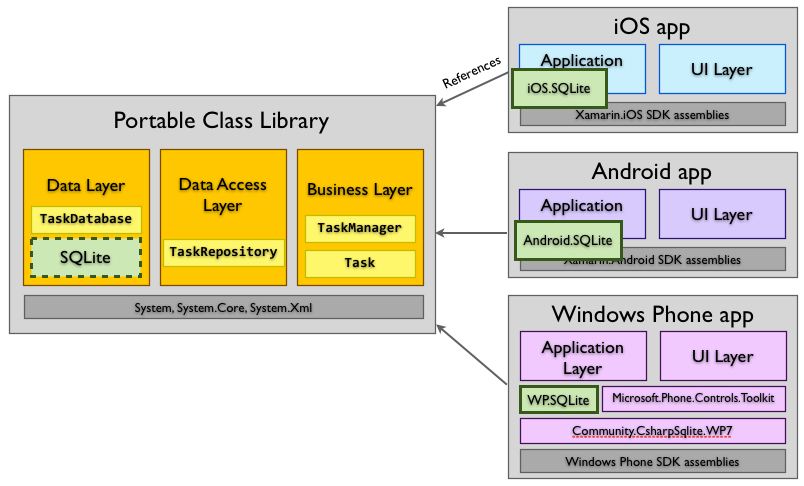
\includegraphics[scale=0.40]{immagini/progettazione/PortableClassLibrary.png}
	\caption{\textit{Architettura Xamarin.Forms PCL}}
\end{figure}\FloatBarrier

Vi sono diversi pro e contro nell'utilizzo delle PCL:
\begin{itemize}
	\item \textbf{PRO:} condivisione del codice centralizzata: il codice scritto e testato all'interno di un progetto singolo può poi essere riutilizzato da altre librerie o applicazioni.
	\item \textbf{PRO:} effettuando il \textit{Refactoring\ped{G}} viene modificato tutto il codice caricato nella soluzione, sia nella \textit{PCL\ped{G}}che nei progetti specifici per piattaforma.
	\item \textbf{PRO:} il progetto \textit{PCL\ped{G}} può essere facilmente referenziato da altri progetti in una soluzione, oppure l'\textit{assembly\ped{G}} risultante può essere condiviso perché altri lo referenzino nelle loro soluzioni.
	\item \textbf{CONTRO} la \textit{PCL\ped{G}} potendo essere condivisa con diverse applicazioni, le librerie specifiche per la piattaforma non possono essere riferite direttamente.
	\item \textbf{CONTRO} la \textit{PCL\ped{G}} non può includere classi fruibili contemporaneamente in \textit{MonoTouch\ped{G}} e \textit{Mono for Android\ped{G}}. 
\end{itemize}
Tuttavia i problemi possono essere parzialmente risolti sfruttando il \textit{Dependency Service\ped{G}} provvisto da Xamarin, che consente di codificare implementazioni specifiche per piattaforma in un' \textit{interfaccia\ped{G}} definita nella \textit{PCL\ped{G}}.
\subsubsection{Shared project}
Contrariamente agli altri approcci, un progetto condiviso non risulta inserito nella creazione di una \textit{DLL\ped{G}}; il codice viene invece compilato in ciascun progetto che lo referenzia, facendo in modo che ogni progetto condiviso referenziato venga compilato come se fosse dello stesso.
\\
Un progetto consiviso può contenere direttiveche ne disabilitano alcune sezioni, secondo la piattaforma su cui viene eseguito il codice.

\begin{figure}[ht]
	\centering
	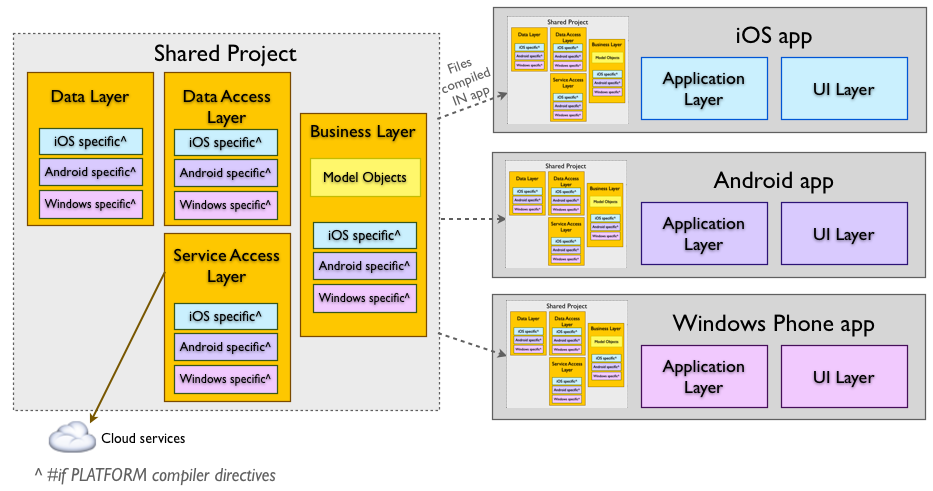
\includegraphics[scale=0.39]{immagini/progettazione/SharedAssetProject.png}
	\caption{\textit{Architettura Xamarin.Forms Shared Project}}
\end{figure}\FloatBarrier

Poichè un progetto condiviso non può essere compilato singolarmente, ma va effettivamente inserito nei progetti che lo referenziano, non può a sua volta referenziare altri progetti, nemmeno altri progetti condivisi.

\subsubsection{Approccio scelto}

Per lo sviluppo dell'applicativo è stato scelto di adottare l'approccio \textit{cross-platform\ped{G}} basato su \textit{PCL\ped{G}}; infatti, considerato che il codice scritto deve essere fruibile da ogni \textit{sistema operativo\ped{G}}, compilare parti specifiche per ogni piattaforma avrebbe complicato l'architettura del progetto. 
\subsection{Progettazione dell'interfaccia grafica}
Xamarin.Forms fornisce una singola \textit{API\ped{G}} per lo sviluppo di \textit{UI\ped{G}}, che traduce a \textit{runtime\ped{G}} i controlli di Xamarin.Forms negli appropriati controlli nativi della piattaforma, per poi renderizzarli.
\\
Per la creazione di \textit{UI\ped{G}}, sono fornite \textbf{quattro classi} principali, che possono essere combinate per realizzare le interfacce desiderate:
\begin{enumerate}
	\item \textbf{Page:} è un elemento visuale che ricopre totalmente, o quasi, lo schermo del dispositivo e contiene una singolo foglio.
	
	\begin{figure}[ht]
		\centering
		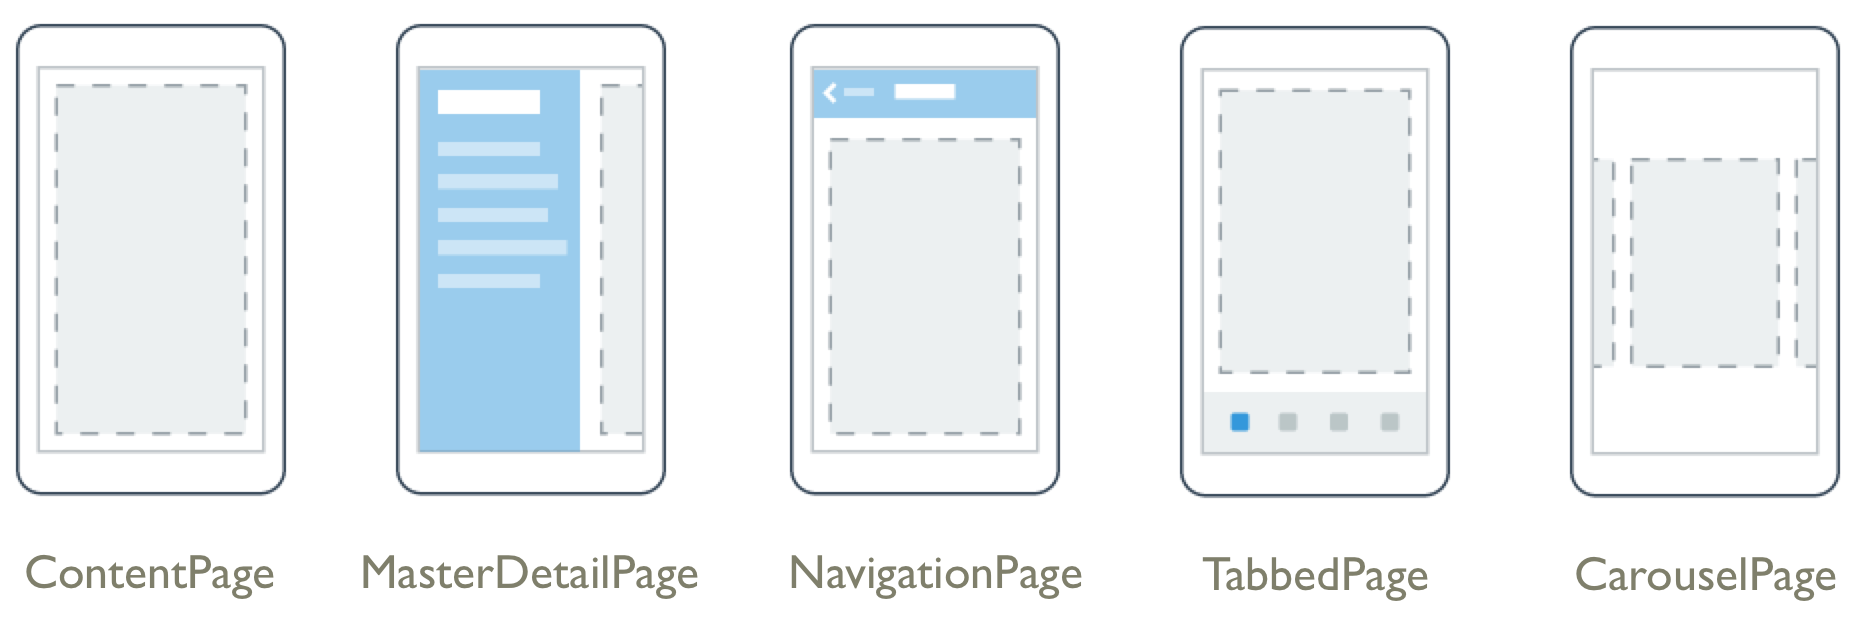
\includegraphics[scale=0.30]{immagini/progettazione/page-types.png}
		\caption{\textit{Tipi di Page fornite da Xamarin.Forms}}
	\end{figure}\FloatBarrier
	
	\item \textbf{Layout:} sono una specializzazione della classe \textbf{View}; fungono da contenitori per altri \textit{Layout\ped{G}} o controlli e vengono utilizzati per gestireil posizionamento e la dimensione dei contenuti.
	
		\begin{figure}[ht]
			\centering
			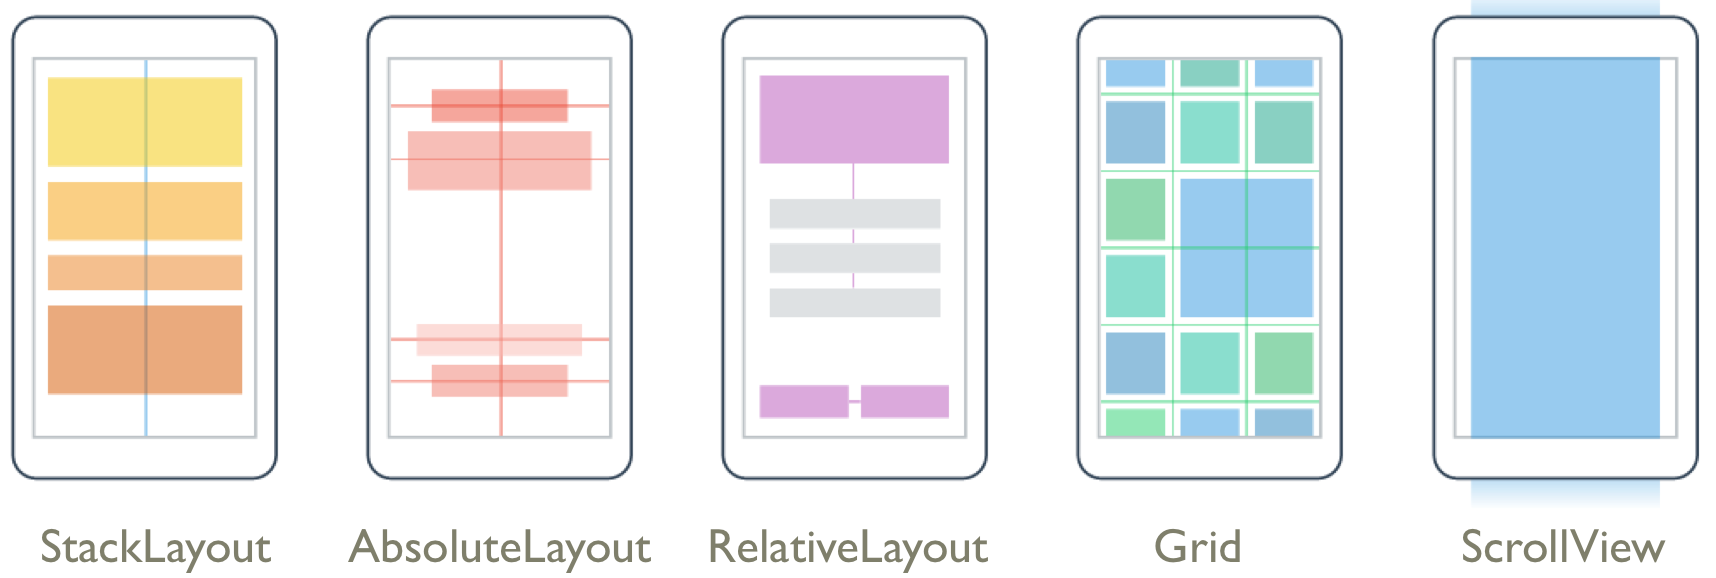
\includegraphics[scale=0.33]{immagini/progettazione/Layouts.png}
			\caption{\textit{Tipi di Layout forniti da Xamarin.Forms}}
		\end{figure}\FloatBarrier
		
		\item \textbf{View:} sono definiti \textit{View\ped{G}} tutti gli elementi grafici, come i pulsanti, le etichette, gli inserimenti di testo. Tutti questi elementi vengono coordinati allo stile grafico tipico della piattaforma usata.
		
		\item \textbf{Cells:} è un elemento usato per realizzare oggetti nelle liste o nelle tabelle e specifica come ogni oggetto nella lista deve essere visualizzato. Una cella dunque non è un elemento grafico, ma una struttura per creare diversi elementi grafici, fornendo le caratteristiche di base di ogni cella
		
\end{enumerate}

\subsection{Data Binding}
Xamarin.Forms usa il \textit{Data-Binding} per semplificare come le interfacce utente delle applicazioni interagiscono con i dati sottostanti. 
\\
Il \textit{Data-Binding\ped{G}} definisce la relazione tra due oggetti, la sorgente provvede i dati mentre il bersaglio li usa, solitamente mostrandoli a video. Nel progetto è stato usato un \textit{framework\ped{G}} per semplificare l'utilizzo di \textit{MVVM\ped{G}} con il \textit{Data-Binding\ped{G}}. \textit{MVVMLight\ped{G}} permette di avere delle strutture già pronte che permettono facilmente di collegare le \textit{Property\ped{G}} dei \textit{ViewModel\ped{G}} con le componenti grafiche per eseguire il \textit{Data-Binding\ped{G}}.

\subsection{Accesso a funzioni native}
Nell'applicativo spesso si deve richiedere delle funzioni specifiche della piattaforma. In un progetto \textit{PCL\ped{G}} non è possibile scrivere codice nativo direttamente nel progetto portabile, si deve dunque utilizzare delle tecniche per richiamare metodi scritti nel codice nativo della piattaforma.
 
\subsubsection{Dependency Service}
Xamarin.Forms fornisce un semplice metodo per implementare funzionalità native delle piattaforme che non sono facilmente condivisibili tra loro, il \textit{Dependency Service\ped{G}}, e il suo funzionamento prevede tre parti:
\begin{itemize}
	\item \textbf{Interfaccia:} una classe interfaccia nel codice condiviso che definisce le funzionalità che richiedono codice specifico per la piattaforma.
	\item \textbf{Registrazione:} un'implementazione dell'interfaccia in ogni progetto dell'applicazione, con allegato un attributo che registri la classe in modo che il \textit{Dependency Service\ped{G}} possa crearne istanze.
	\item \textbf{Locazione:} chiamando il \textit{Dependency Service\ped{G}} nel codice condiviso si ottinene a runtime un'istanza dell'interfaccia definita, consentendo al codice condiviso di accedere alla piattaforma sottostante.
\end{itemize}

\subsection{Design Pattern}
Durante la fase di progettazione, è stato considerato il \textit{design pattern\ped{G}} architetturale \textit{Model-View-ViewModel} per la separazione della grafica dal contenuto e per semplificare la connessione tra le componenti.
\subsubsection{Model-View-ViewModel}
Il \textit{Model-View-ViewModel\ped{G}} è un \textit{design pattern\ped{G}} architetturale creato da \textit{Microsoft\ped{G}} nel 2005, pensato inizialmente per aiutare lo sviluppo di applicativi \textit{WPF\ped{G}} e \textit{Silverlight\ped{G}}, sfruttando le funzioni di \textit{Data-Binding\textit{G}}.
\\
\textit{MVVM\ped{G}} consente, associato a \textit{XAML\ped{G}}, di sviluppare \textit{UI\ped{G}} in modo completamente indipendente dalla logica, collegando i campi da popolare alla struttura sottostante con \textit{Data-Binding\ped{G}}. Questa profonda separazione tra grafica e logica rende indipendente lo sviluppo delle due parti, semplificando la strutturazione della parte grafica degli applicativi.

\paragraph{Model}
Il model è un'implementazione del \textit{domain model\ped{G}} dell'applicazione, il quale include i dati e la loro logica di business e validazione. Questi sono rappresentanti quindi sia da \textit{database\ped{G}} o altri archivi, sia da oggetti di accesso ai dati.
\paragraph{View}
La View rappresenta l'interfaccia grafica con cui l'utente interagisce, limitandosi a presentare i dati richiesti ed i controlli necessari per gestirli. La View in \textit{MVVM\ped{G}} è attivae gestiche comportamenti, eventi e \textit{Data-Binding\ped{G}} che richiedono una conoscenza del Model sottostante, solitamente mappandoli a proprietà o comandi.
\paragraph{ViewModel}
Il ViewModel si frappone tra View e Model, occupandosi delle iterazioni tra i due, facendo in modo che il Model non venga influenzato da come la View gestisce i suoi dati ed impedendo alla View una connessione diretta con il Model. Il ViewModel espone metodi, dati e comandi neccessari alla View, rispondendo ai suoi \textit{input\ped{G}} con chiamate ai metodi del Model, traducendone i risultati in formati fruibili e lanciando eventi perché la View li utilizzi. Se il Model viene modificato, invia eventi al ViewModel perché ne rilevi le modifiche e faccia in modo che la View agisca di conseguenza.

		\begin{figure}[ht]
			\centering
			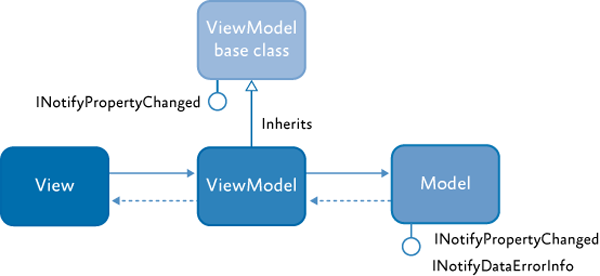
\includegraphics[scale=0.45]{immagini/progettazione/IC448599.png}
			\caption{\textit{Componenti Model-View-ViewModel}}
		\end{figure}\FloatBarrier

\section{Diagramma delle classi}
Al termine della fase di progettazione è stato prodotto uno schema delle classi che è rimasto circoscritto alla libreria condivisa, nel quale è stato cercato di evidenziare l'implementazione del pattern \textit{MVVM\ped{G}}.
\\
Ogni piattaforma contiene un file main, che permette di accedere alla libreria condivisa e creare la \textit{Classe App\ped{G}}, allo scopo di inizializzare l'applicazione.
\\
I componenti dell'applicazione \app sono i componenti imposti dal \textit{design pattern\ped{G}} architetturale \textit{Model-View-ViewModel\ped{G}}
		\begin{figure}[ht]
			\centering
			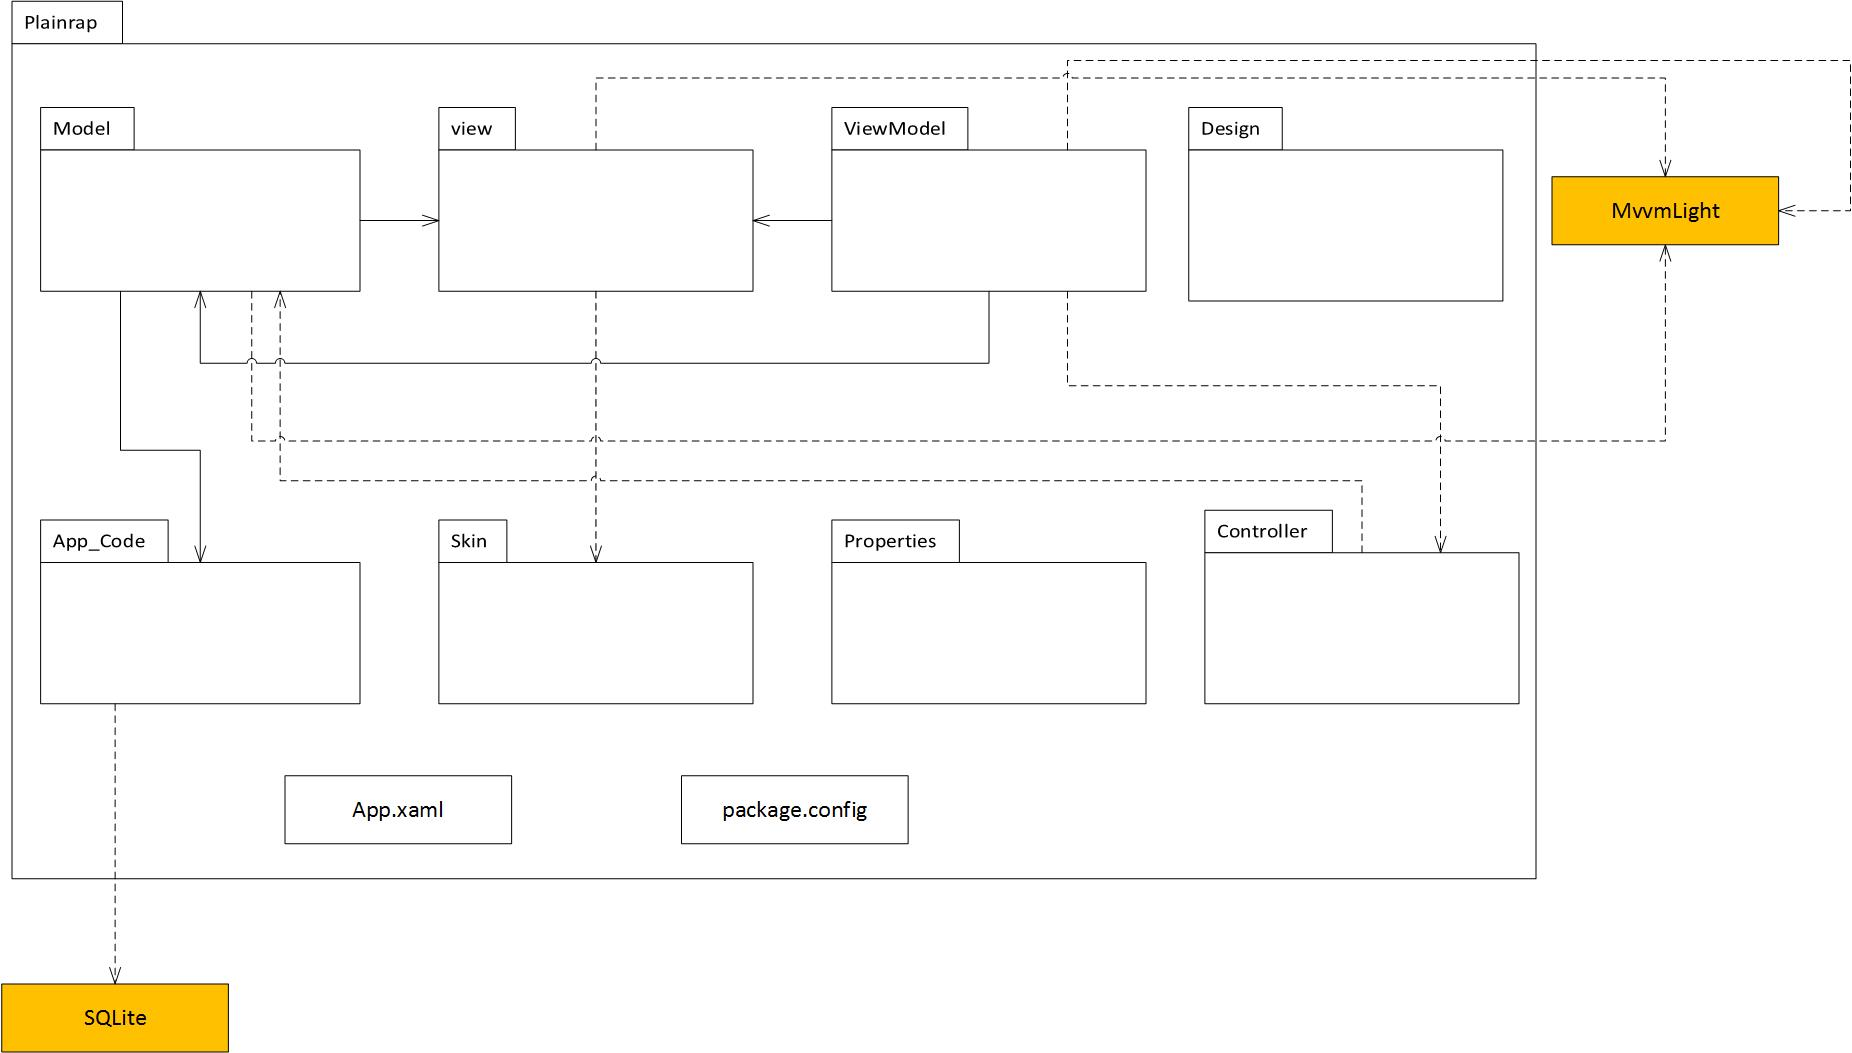
\includegraphics[scale=0.38]{immagini/progettazione/plainrap_portable.jpg}
			\caption{\textit{Componenti Plain.Rap.Mobile}}
		\end{figure}\FloatBarrier

\section{Strumenti utilizzati}
\subsection{Ambiente di sviluppo}
Per sviluppare l'applicativo è stato utilizzato l'ambiente di sviluppo \textit{Visual Studio\ped{G}}, in quanto è l' \textit{IDE\ped{G}} standard impiegato da \asi.

\subsection{Pacchetti NuGet}
NuGet èun gestoredi pacchetti per le piattaforme di sviluppo \textit{Microsoft\ped{G}} e \textit{.NET\ped{G}}, i pacchetti NuGet contengono librerie o strumenti che forniscono funzionalità indipendenti dal progetto in cui possono essere applicate, ogni pacchetto NuGetcontiene i file da copiare ed un manifesto che ne spiega i contenuti e definisce come aggiungerlo o rimuoverlo.
\\
Quando si vuole installare un pacchetto, NuGet copia i file nella soluzione e automaticamente aggiorna i riferimenti. Alla rimozione, NuGet rimuove i file ed i riferimenti assegnati all'installazione, pulendo di fatto il progetto.

\subsubsection{SQLite.Net}
Questo pacchetto NuGet installa nel progetto le funzionalità necessarie alla creazione e gestione di un database \textit{SQLite\ped{G}} consentendo anche l'accesso asincrono ai dati, per non bloccare l'applicativo durante tali operazioni.
\\
Il pacchetto è stato usato per gestire il database locale all'interno del dispositivo, inserito in ogni piattaforma, e richiamato tramite \textit{Dependency Service\ped{G}}.

\subsubsection{Newtonsoft.Json}
Questo pacchetto offre un semplice \textit{framework\ped{G}} per la \textit{serializzazione} e la \textit{deserializzazione} di documenti in formato \textit{.json\ped{G}} da oggetti del model.
\\
La necessità di utilizzare il formato \textit{.json} è data dalla funzionalità di sincronizzazione, che avviene attraverso dei servizi \textit{REST\ped{G}} esposti da un servizio creato ad hoc.

\subsubsection{iTextSharp}
La conversione in \textit{PDF\ped{G}} dopo la trasformata \textit{XSLT\ped{G}} avviene grazie le funzionalità fornite da questo pacchetto, nella sua versione apposita per \textit{Xamarin\ped{G}}. Attualmente il \textit{parser\ped{G}} per la trasformata è obsoleto, ecludendo di fatto alla piena potenzialità del template \textit{XSLT}

\subsubsection{MVVMLight}
Questo pacchetto, sviluppato da \textit{GalaSoft\ped{G}}, aiuta lo sviluppo su \textit{design pattern\ped{G}} architetturale \textit{Model-View-ViewModel\ped{G}}, fornendo un sistema pronto di locazione dei \textit{ViewModel\ped{G}} e un sistema di messaggistica per diminuire la dipendenza tra classi.

\subsection{Emulator Android for Visual Studio}
Per il \textit{Debug\ped{G}} durante lo sviluppo è stato utilizzato un emulatore \textit{Android\ped{G}} sviluppato per \textit{Visual Studio\ped{G}}. L'emulatore presenta una grossa comodità, sopratutto per la varietà di configurazioni possibili in termini di \textit{Hardware\ped{G}} e di versione di \textit{Sistema operativo\ped{G}}.


